\section{Application: H$_2$/O$_2$ Reaction Kinetics}
\label{sec:app}

%Problem set-up: something about the reaction - why is it important?
%different reactions, reaction rate definition, uncertain parameters,
%quantity of interest. 
%
%Implementation of the proposed methodology for two scenarios: lean
%mix and rich mix. Describe what we mean by lean and rich using
%stoichiometry. 
%
%Define all the inputs as per the framework and illustrate its
%implementation to this application for both scenarios

The proposed framework in section~\ref{sec:method} is implemented to 
the H$_2$/O$_2$ reaction mechanism provided in~\cite{Yetter:1991}.
The mechanism comprises of 19 reactions including chain reactions,
dissociation/recombination reactions, and formation and consumption
of intermediate species: HO$_2$ and H$_2$O$_2$, as provided below
in Table~\ref{tab:kinetics}.

\begin{table}[htbp]
\renewcommand*{\arraystretch}{1.2}
\begin{center}
\begin{tabular}{llll}
\toprule
Reaction \#     & Reaction &&\\
\bottomrule
$\mathcal{R}_1$ & H + O$_2$          & $\rightleftharpoons$ & O + OH \\
$\mathcal{R}_2$ & O + H$_2$          & $\rightleftharpoons$ & H + OH \\
$\mathcal{R}_3$ & H$_2$ + OH         & $\rightleftharpoons$ & H$_2$O + H \\
$\mathcal{R}_4$ & OH + OH            & $\rightleftharpoons$ & O + H$_2$O \\
$\mathcal{R}_5$ & H$_2$ + M          & $\rightleftharpoons$ & H + H + M \\
$\mathcal{R}_6$ & O + O + M          & $\rightleftharpoons$ & O$_2$ + M \\
$\mathcal{R}_7$ & O + H + M          & $\rightleftharpoons$ & OH + M \\
$\mathcal{R}_8$ & H + OH +M          & $\rightleftharpoons$ & H$_2$O + M \\
$\mathcal{R}_9$ & H + O$_2$ + M      & $\rightleftharpoons$ & HO$_2$ + M \\
$\mathcal{R}_{10}$ & HO$_2$ + H      & $\rightleftharpoons$ & H$_2$ + O$_2$ \\
$\mathcal{R}_{11}$ & HO$_2$ + H      & $\rightleftharpoons$ & OH + OH \\
$\mathcal{R}_{12}$ & HO$_2$ + O      & $\rightleftharpoons$ & O$_2$ + OH \\
$\mathcal{R}_{13}$ & HO$_2$ + OH     & $\rightleftharpoons$ & H$_2$O + O$_2$ \\
$\mathcal{R}_{14}$ & HO$_2$ + HO$_2$ & $\rightleftharpoons$ & H$_2$O$_2$ + O$_2$ \\
$\mathcal{R}_{15}$ & H$_2$O$_2$ + M  & $\rightleftharpoons$ & OH + OH + M \\
$\mathcal{R}_{16}$ & H$_2$O$_2$ + H  & $\rightleftharpoons$ & H$_2$O + OH \\
$\mathcal{R}_{17}$ & H$_2$O$_2$ + H  & $\rightleftharpoons$ & HO$_2$ + H$_2$ \\
$\mathcal{R}_{18}$ & H$_2$O$_2$ + O  & $\rightleftharpoons$ & OH + HO$_2$ \\
$\mathcal{R}_{19}$ & H$_2$O$_2$ + OH & $\rightleftharpoons$ & HO$_2$ + H$_2$O \\
\bottomrule
\end{tabular}
\end{center}
\caption{Reaction mechanism for H$_2$/O$_2$ from~\cite{Yetter:1991}}.
\label{tab:kinetics}
\end{table}


The reaction rate for the $i^{th}$ reaction as a function of temperature
is given as follows:
\be
k_i(T) = A_iT^{n_i}\exp(-E_{a,i}/RT), 
\label{eq:rate}
\ee
%
where $A_i$ is the pre-exponent, $n_i$ is the index of $T$, $E_{a,i}$ is the
activation energy corresponding to the $i^{th}$ reaction, and $R$ is the
universal gas constant. We focus on quantifying the uncertainty in the
\emph{ignition delay} due to uncertainty associated with the pre-exponent,
$A_i$ for each reaction. Hence, the total number of uncertain parameters in the
present case is 19.  The $A_i$'s are considered to be uniformly distributed in
the interval: $[0.9A_i^\ast, 1.1A_i^\ast]$; $A_i^\ast$ being the nominal
estimate corresponding to the $i^{th}$ reaction. TChem~\cite{Safta:2011}, an
open source C package was used for simulating temperature and concentration
evolution during the progress of reactions $\mathcal{R}_1$--$\mathcal{R}_{19}$,
and determining the ignition delay. The set of nominal values used in the
computations, for parameters in~\eqref{eq:rate} are provided
in~\cite{Yetter:1991}. 

While the dimensionality of the problem is relatively moderate,
constructing a surrogate in the 19-dimensional parameter space could still be
expensive. Hence, we explore the possibility of constructing a
reduced-space surrogate (RSS) using the framework presented 
in section~\ref{sec:method}. 
In the present study, we focus on two scenarios: fuel(H$_2$)-rich, and
fuel(H$_2$)-lean. Consider the global reaction:
%
\be
2\text{H}_2 + \text{O}_2 \rightarrow 2\text{H}_2\text{O}
\label{eq:global}
\ee 
%
The equivalence ratio $\phi$ is defined as follows:
%
\be
\phi = \frac{(M_{\text{H}_2}/M_{\text{O}_2})_\text{obs}}{(M_{\text{H}_2}/M_{\text{O}_2})_\text{st}}
\label{eq:phi}
\ee
%
The numerator in the right-hand-side represents the observed (obs) fuel-oxygen
mass ratio at a given condition and the denominator represents the
stoichiometric (st) ratio of the same quantity. Hence, $\phi$ = 1 at
stoichiometric conditions. The equivalence ratio can be altered by changing the
amount of O$_2$ in the mixture. In the case of a lean
mixture,~\eqref{eq:global} can be written as follows:
%
\be
2\text{H}_2 + \alpha\text{O}_2 \rightarrow 2\text{H}_2\text{O} + (\alpha-1)\text{O}_2 
\hspace{3mm} (\alpha>1)
\label{eq:lean}
\ee 
%
Similarly, for the case when the mixture if fuel rich,~\eqref{eq:global} is modified
as follows:
%
\be
2\text{H}_2 + \alpha\text{O}_2 \rightarrow 2\alpha\text{H}_2\text{O} + 2(1-\alpha)\text{H}_2
\hspace{3mm} (\alpha<1)
\label{eq:rich}
\ee 
%
Eqs.~\eqref{eq:lean} and~\eqref{eq:rich} can be generalized as follows:
%
\be
2\text{H}_2 + \alpha\text{O}_2 \rightarrow 2\min(1,\alpha)\text{H}_2\text{O} + 
\max(\alpha-1,0)\text{O}_2 + \max(0,2-2\alpha)\text{H}_2
\label{eq:gen}
\ee 
%
From the above set of chemical equations, the relationship between $\phi$
and $\alpha$ can be easily obtained as $\phi~=~\frac{1}{\alpha}$.
Since $\phi>1$ corresponds to a rich mixture, and $\phi<1$ corresponds to a
lean mixture, we consider $\phi$ = 2.0 and 0.5 to investigate the two scenarios
respectively. 

We apply the parameter screening algorithm with the following
parameters: $\tau_\text{screen}$, $s_\text{min}$,
$s_\text{max}$, $\beta$ are fixed at 0.2, 3, 10, and 1.0 respectively for both cases.
Additionally, the value of $\tau$ is considered to be 1.0$\times 10^{-17}$ and
5.0$\times 10^{-17}$ in the rich and lean case respectively. Such a small value
of $\tau$ for this application is a consequence of the nature of convergence exhibited
by the sensitivity measures. Moreover, the screening procedure is carried out
for atleast $s_\text{min}$ number of iterations in order to bolster our confidence
in the estimates. 

Following the steps outlined in the flow-diagram in Figure~\ref{fig:flow}, model
evaluations are initially generated at $n_1$ = 5 samples. The evaluations are
used to construct a regression-based surrogate in the full-space. As
expected, the surrogate is found to be highly inaccurate. Moreover, unlike the
test problems in section~\ref{sec:examples}, we do not estimate the Sobol
total-effect sensitivity indices in the interest of following the overall framework
closely. Hence, we proceed to the screening step to estimate the screening metric
for the uncertain pre-exponents, $A_i$'s. Results are plotted below
in Figure~\ref{fig:sense_kinetics}~(top row) for both cases. Furthermore, we illustrate
the decay in the value of $\Delta\mu_s$ with iterations in 
Figure~\ref{fig:sense_kinetics}~(bottom row). 

\begin{figure}[htbp]
 \begin{center}
  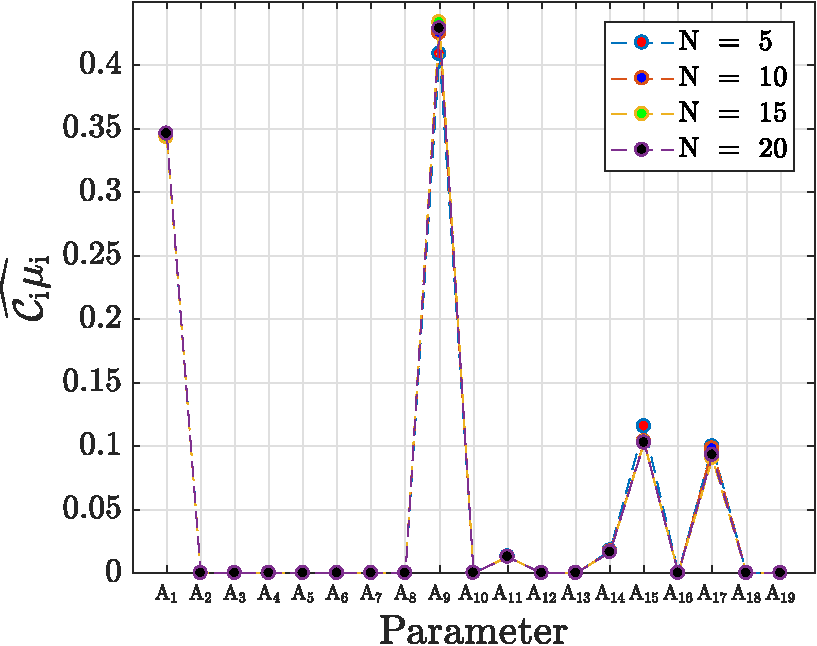
\includegraphics[width=0.48\textwidth]{./Figures/ub_conv_kinetics_rich}
  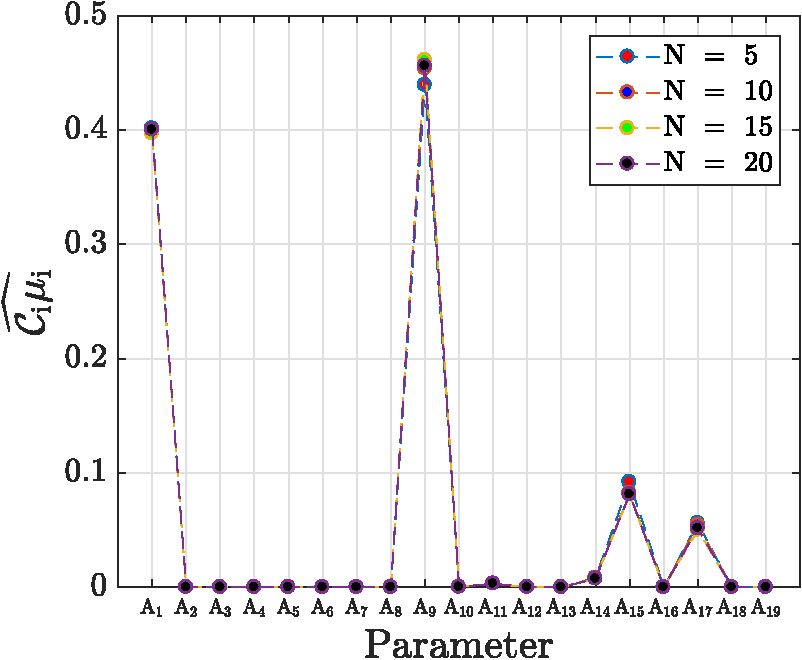
\includegraphics[width=0.48\textwidth]{./Figures/ub_conv_kinetics_lean}
  \\ \vspace{2mm}
  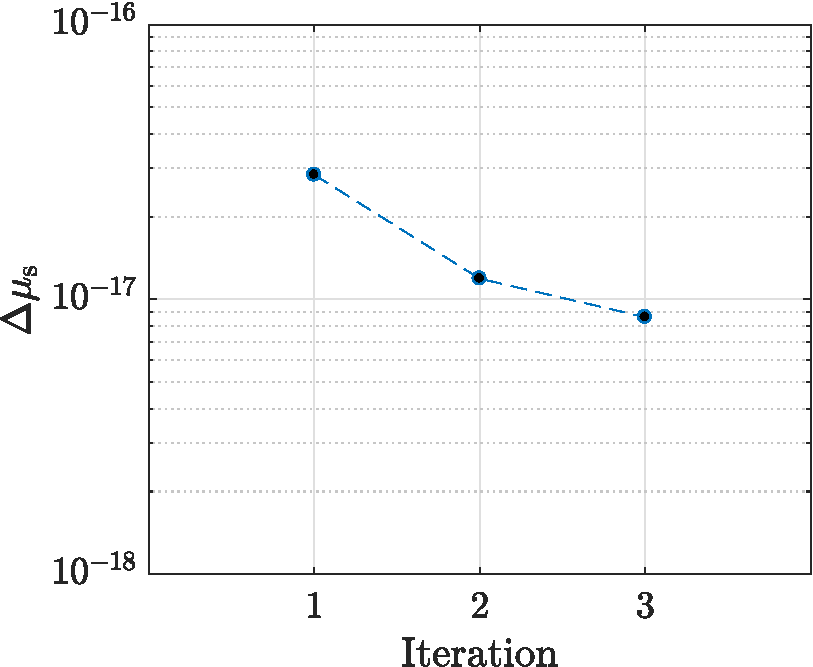
\includegraphics[width=0.48\textwidth]{./Figures/mu_rich}
  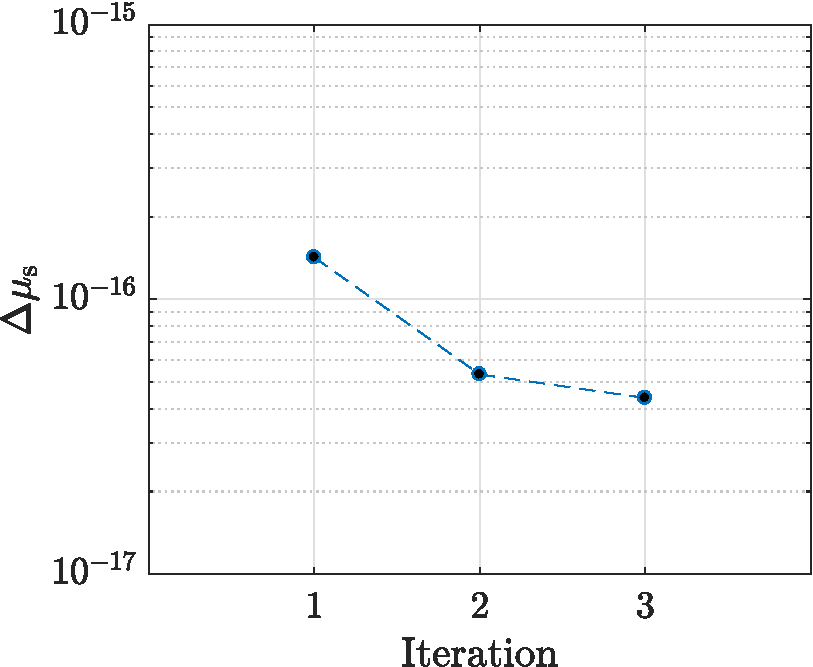
\includegraphics[width=0.48\textwidth]{./Figures/mu_lean}
\caption{Top: Estimates of $\widehat{\mathcal{C}_i\mu_i}$ for $A_i$'s in the case
of fuel-rich mixture~(left) and fuel-lean mixture~(right). Bottom: The value of
$\Delta\mu_s$ during three iterations within the screening step are plotted for
the case of fuel-rich mixture~(left) and fuel-lean mixture~(right).}
\label{fig:sense_kinetics}
\end{center}
\end{figure}
%
The screening metric estimates in the above plots are observed to converge with
only a few samples (5--10). Moreover, out of the 19 uncertain pre-exponents,
only $A_1$, $A_9$, $A_{15}$, and $A_{17}$ seem to be important in the fuel-rich
case, whereas, only $A_1$, $A_9$, and $A_{15}$ seem important in the fuel-lean
case, based on the value of $\tau_\text{screen}$. These observations are indicative
of the potential for significant reduction in the dimensionality of this problem. 
A reduced-space
surrogate constructed using the proposed framework could thus lead to large computational
gains. The decay of $\Delta\mu_s$ with iterations is expected and builds our confidence
in the screening procedure in both cases.

A reduced-space surrogate (RSS) was constructed in 4D for the fuel-rich case,
and in 3D for
the fuel-lean case. Figure~\ref{fig:err_samples_kinetics} illustrates a
comparison of convergence characteristics for the PCEs constructed in the
full-space and the reduced-space for the fuel-rich case. Note that the
plot is generated using the implementation of least angle regression (LAR)
for sparse PCEs in UQLab.  
%
\begin{figure}[htbp]
 \begin{center}
  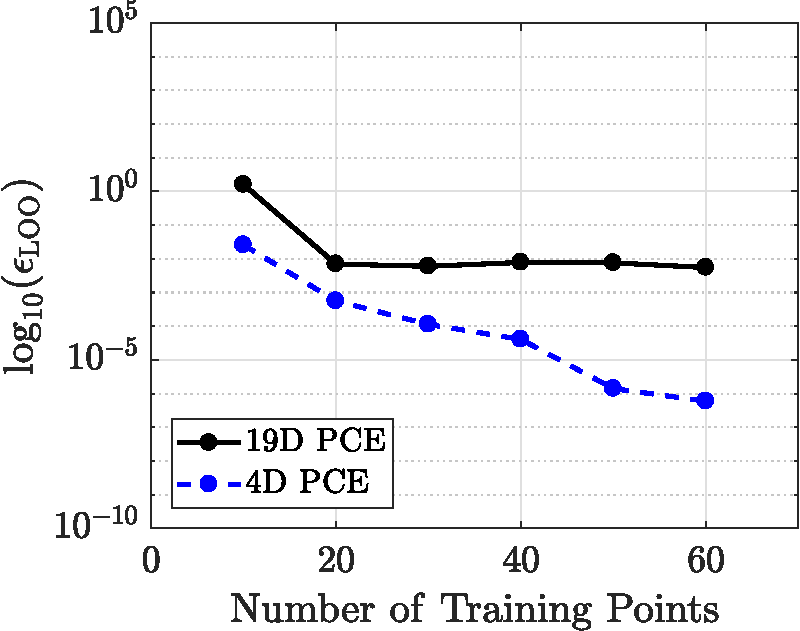
\includegraphics[width=0.48\textwidth]{./Figures/err_samples_kinetics}
\caption{A semi-log plot of $\epsilon_\text{\tiny LOO}$ as a function of
number of model evaluations in the full-space (19D) and the reduced-space (4D)
for the fuel (H$_2$)-rich case i.e. $\phi$ = 2.0.}
\label{fig:err_samples_kinetics}
\end{center}
\end{figure}
%
The leave-one-out cross validation error is observed to drop initially
and plateau with the increase in training points for the 19-dimensional
PCE. However, in the case of 4-dimensional PCE, the error exhibits a
monotonic behavior and is found to be smaller than $\mathcal{O}(10^{-5})$
at 60 training points. Clearly, the RSS shows a much faster rate of convergence.
Similar trends (not included) were observed in the fuel-lean case. 

Based on $\epsilon_{\mbox{\tiny{L-2}}}$ estimates using the 
cross-validation set, the RSS was found to be accurate within 1.8$\%$ in the
fuel-rich case, and
within 3.1$\%$ in the fuel-lean case. Model evaluations at 1000 samples in the test suite
are further used to plot a normalized histogram of the ignition time in 
Figure~\ref{fig:pdf_kinetics}. To verify the accuracy of the RSS in a 
probabilistic-sense, we compare the histogram plot with a PDF of ignition time
using surrogate predictions at 10$^{6}$ samples in the reduced space in both cases. 
%
\begin{figure}[htbp]
 \begin{center}
  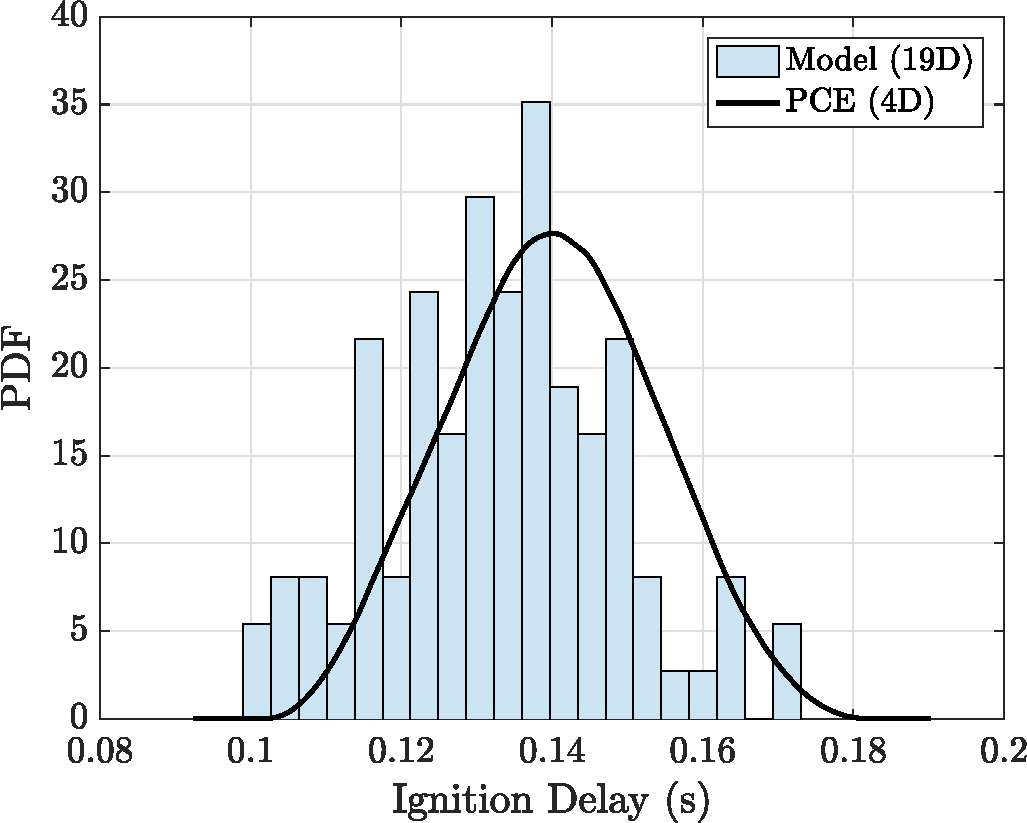
\includegraphics[width=0.48\textwidth]{./Figures/pdf_comp_rich}
  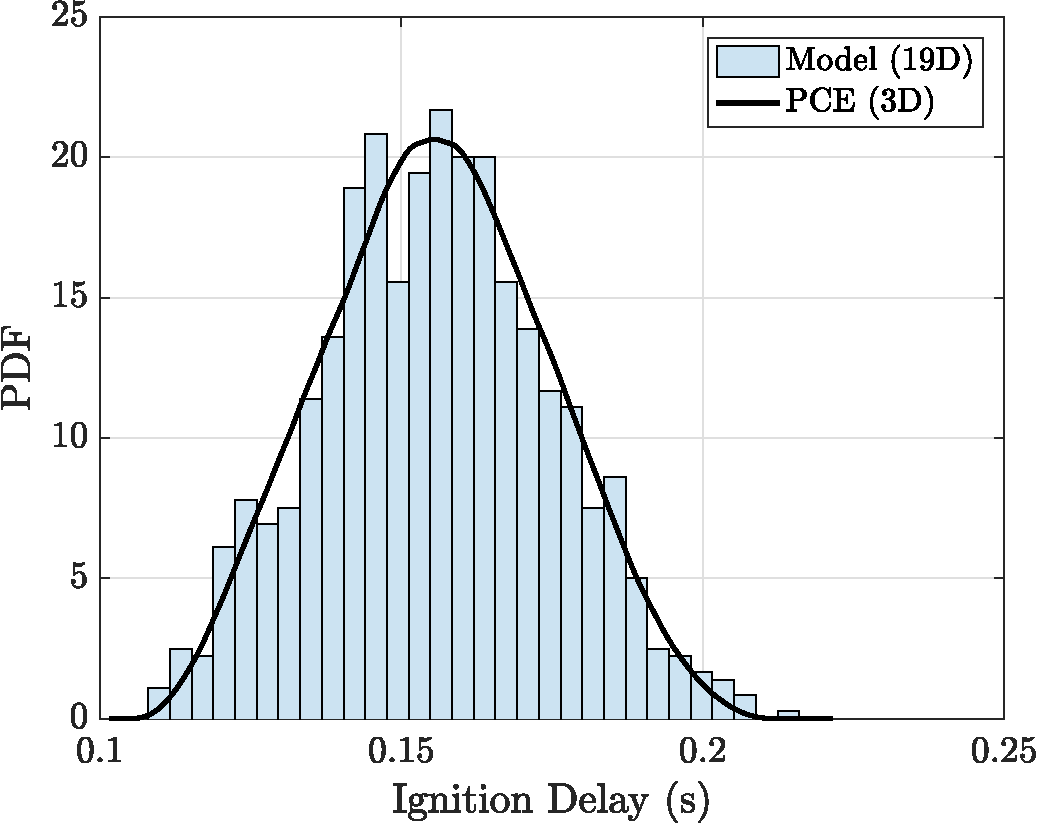
\includegraphics[width=0.48\textwidth]{./Figures/pdf_comp_lean}
\caption{A normalized histogram based on model evaluations at 1000 samples is plotted
along with a PDF of ignition delay for the fuel-rich case (left) and the fuel-lean
case (right).}
\label{fig:pdf_kinetics}
\end{center}
\end{figure}
%
Clearly, the RSS captures the spread as well as the modal estimate of
the ignition delay in both scenarios. Hence, the proposed framework 
has enabled significant dimension reduction and construction of an accurate
RSS for multiple scenarios pertaining to the H$_2$/O$_2$ reaction
mechanism.    
